\section{Results}

\subsection{Do the assays work? A dyad that is communicating by construction}
\label{sec:assay}

Every negative result below rests on an assay reporting ``no communication
here''. An assay that reported that unconditionally would produce the same
paper, so before applying them we check that they fire on a case where
communication is not in question.

We embed a Lewis signalling game in the same physics. One fish is immobile and
privately observes which of two sites holds food; the other must travel to a
site. The sender's discharges are forced onto a fixed schedule, so pulse timing
carries nothing, and the only free channel is a one-bit discharge subtype. Both
fish are scored on the receiver reaching the correct site, and the harvest is
shared. Crossing an informative sender (subtype $=$ the private cue) against an
uninformative one (a bit that is constant within a trial but uncorrelated with
the truth), and a receiver that attends to the subtype against one that ignores
it, gives four dyads whose communication status we know
(Fig.~\ref{fig:assay}). Only the informative-and-attended dyad succeeds:
\AssayArrHonest\ correct arrivals out of four per episode, against \AssayArrDeaf\
for chance.

Each assay behaves as it should, and---more usefully---each one alone is
foolable. Positive signalling is \AssayMIHonest\ bits for the informative sender
and \AssayMIRandom\ for the uninformative one, but it is just as high when
nobody is listening, because it measures the sender in isolation. Causal
influence and positive listening separate the attending receiver from the deaf
one (\AssayCIEListen\ versus \AssayCIEDeaf\ nats) but are just as high when the
channel carries nothing, because a receiver can organise its behaviour around a
variable that is pure noise. Even the payoff test is foolable on its own:
deleting the subtype costs the attending receiver \AssayKillHonest\ when the
subtype is informative and still \AssayKillRandom\ when it is noise, because the
receiver has come to depend on it either way.

Only the conjunction identifies communication. This is the standard we hold the
electric discharge to in what follows, and it is a standard the discharge could
in principle meet: the instruments are demonstrably capable of detecting a
payoff-relevant, informative, attended channel in this simulator.

\begin{figure}[t]
\centering
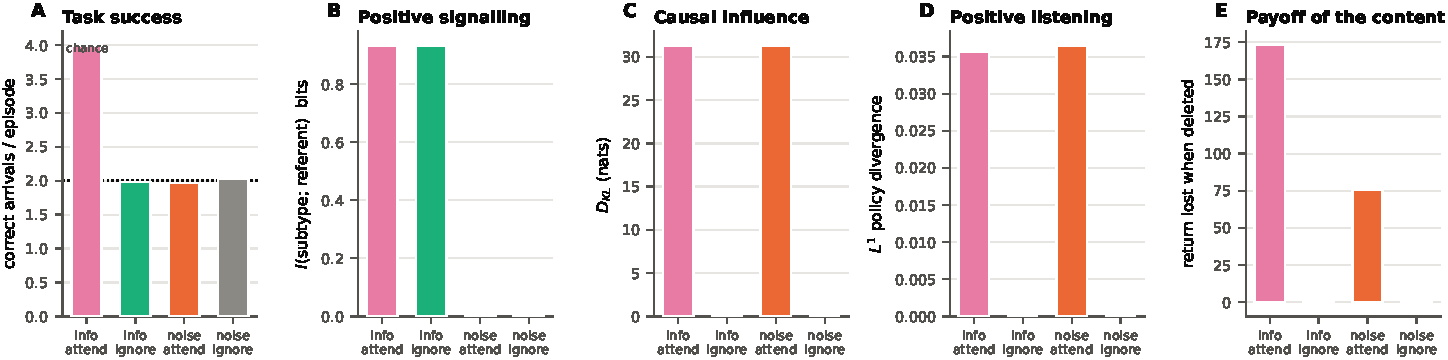
\includegraphics[width=\textwidth]{../figs/fig0_assay_validation.pdf}
\caption{\textbf{The assays detect communication when it is present, and each is
foolable alone.} Four dyads in the referential game. Only \emph{info+attend} is
communicating; the other three each satisfy some subset of the diagnostics.}
\label{fig:assay}
\end{figure}

\subsection{What the optimiser can and cannot do}
\label{sec:optimiser}

A negative result about communication invites the objection that the learner, not
the environment, is the limiting factor. We measured this rather than argued about
it, because the answer bounds what the rest of the paper may claim.

In the same referential game we trained recurrent MAPPO under three conditions,
twelve seeds each at \SI{50e6}{} agent-steps: both sides learning; the receiver
learning against a \emph{scripted honest} sender, so the message is already
perfectly informative and only reading it must be discovered; and both sides
learning with the positive-signalling bias of \citet{eccles2019biases}, which
exists to break exactly this deadlock. \emph{None of the thirty-six runs solved
the game}: all sit at chance, against \AssayArrHonest/4 for the hand-coded dyad
reading the same observation vector. Reducing the steering noise by an order of
magnitude and halving the credit horizon do not move it either
(Appendix~\ref{app:optimiser}).

So shared-parameter recurrent MAPPO---the standard configuration, and the one the
reference model uses---does not discover that a single perfectly informative input
bit should select between two known targets in an embodied task, even when told
what to say. Our results therefore divide in two. The muting decomposition, the
foolability of each diagnostic, and the metrics' behaviour under intervention are
measurements on trained policies and do not depend on this. The claims that
metabolic cost fails to create a signal, and that a decoupled channel does not
either, are claims about what learning arrives at and inherit the bound: these
pressures did not produce signalling under a standard learner, not that they could
not under a better one.

\subsection{A validated, fast reimplementation}

The environment is a GPU reimplementation of the reference simulator, checked
stage by stage against the original NumPy code in double precision on random
scenes. All \ValNChecks\ checks agree to floating-point round-off (maximum
relative deviation \ValMaxErr; the knollenorgan and ampullary pathways agree
bit-for-bit), and it sustains \ThroughputK{}k agent-steps per second in aggregate
on two GPUs, which is what makes \NumRuns\ independent training runs affordable.
Appendix~\ref{app:validation} gives the per-stage table and records an incidental
bug in the reference code: its configuration file specifies a wall-reflection
coefficient of $0.95$, but the scene builder never forwards it, so the published
results in fact use unattenuated images.

\subsection{The discharge is worth a great deal --- to the emitter}

Agents that can discharge eat \FullEaten\ food items per episode; agents muted
from the start of training eat \SilentEaten\ (\ProbeGain$\times$, Hedges'
$g=\ProbeD$, $p=\ProbeP$). The probe does real work, which is the precondition
for everything that follows: an \eod\ is not a cheap-talk token but an expensive
and useful act of sensing that happens to be public. Removing the three
consequences one at a time during training orders them---no detection
\NoKnollenEaten, no illumination \NoIllumEaten, private probe only
\PrivateEaten, no reafference \NoSelfEaten---but from-scratch comparisons
confound the value of a channel with the difficulty of learning without it, and
training here is bimodal (Appendix~\ref{app:scratch}). We therefore rely on
interventions applied to frozen policies.

\subsection{The muting effect is almost entirely private sensing}

The central experiment. We take a trained, intact population and, at evaluation
time only, silence one fish---the intervention used upstream---then repeat with
each of its three consequences removed separately. Every condition is run from the
same episode seed, so arena $k$ has the same initial food layout and the same
sensory-noise stream in all of them, and differences are taken within arena.

Muting one fish costs that fish \MuteTargetTotal\ food items per episode
(Fig.~\ref{fig:muting}A). Decomposed: removing only its own reafference costs
\MuteTargetPriv, removing only its illumination of neighbours costs
\MuteTargetCue, and removing only its detectability costs \MuteTargetSig. The
private share accounts for essentially the whole effect.

The effect on its \emph{neighbours} is smaller still (Fig.~\ref{fig:muting}B):
\MuteOthersTotal\ items in total, with the illumination share \MuteOthersCue\
($p=\MuteOthersCueP$) and the detection share \MuteOthersSig\
($p=\MuteOthersSigP$). Group spacing (Fig.~\ref{fig:muting}C) is likewise
unchanged within resolution.

This is the paper's first substantive result, and it is a negative one. When a
fish is silenced in this model, what happens is overwhelmingly that the fish has
been blinded, not that a conversation has been interrupted. An experiment that
reports only the joint effect---as the reference study does, and as \eod-ablation
experiments in real fish must---will attribute to communication an effect that is
almost entirely private electrolocation.

\begin{figure}[t]
\centering
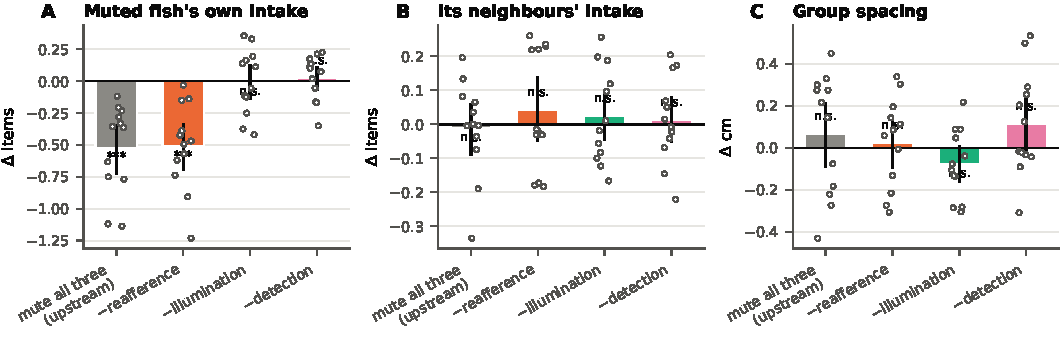
\includegraphics[width=\textwidth]{../figs/fig3_muting_decomposition.pdf}
\caption{\textbf{Silencing one fish removes three things at once; separating them
reassigns the effect.} Within-arena paired differences from the intact channel,
frozen policies. Significance is a permutation test over seeds.}
\label{fig:muting}
\end{figure}

\subsection{The channel nonetheless carries information and moves policies}

It would be wrong to conclude that the public channel is inert. It is not.

Discharge probability depends on the emitter's situation: \EmitFood\ when food is
within \SI{10}{\centi\metre} versus \EmitNoFood\ when it is not
($p=\EmitFoodP$; Fig.~\ref{fig:content}C). That state-dependence is inherited by
the public channel, and a receiver can read it: decoding \emph{only} from the
number of pulses a receiver heard from a given emitter in a trailing window, food
proximity is recovered with $\Delta R^2 = \ContentFood$ above a time-shifted
baseline ($p=\ContentFoodP$; Fig.~\ref{fig:content}B). Positive signalling about
food, measured as mutual information conditioned on distance-to-neighbour decile
so that geometry cannot manufacture it, is \PSFood\ of the state entropy
(Fig.~\ref{fig:content}A).

Positive listening holds too. The interventional causal influence of
Eq.~\ref{eq:cie}---re-rendering a receiver's sensory input under
$\dosim(e_j{=}1)$ versus $\dosim(e_j{=}0)$ with everything else held on its
factual path---is \CIE\ nats, against a noise floor of \CIENull\ nats obtained by
re-rendering the \emph{same} intervention under an independent noise draw
(Fig.~\ref{fig:listening}A). The channel moves receiver policies
\CIERatio$\times$ more than sensory noise does.

Both of these diagnostics, however, behave badly here in ways worth recording.
Positive signalling is \emph{higher} in populations whose receivers are deaf
(\PSDeaf) than in populations whose receivers can hear (\PSHear): a fish
modulates its probe rate with its own situation whether or not anybody is
listening, so the measure is picking up the sensory schedule, not signalling.
This is exactly the artifact \citet{lowe2019pitfalls} warn of, and it is
straightforward to demonstrate once a deaf population is available as a control.
Causal influence misbehaves in the other direction: it \emph{rises}
\CIEFold-fold, from \CIECostZero\ to \CIECostHigh\ nats, as metabolic cost is
increased---that is, precisely as the pulse train becomes rarer and less
informative (Fig.~\ref{fig:listening}D). A rare discharge is more surprising, so
switching it on or off moves the receiver's policy more, even though the train as
a whole now tells the receiver less. Influence per message and information per
unit time are different quantities, and in this system they are
anti-correlated.

\begin{figure}[t]
\centering
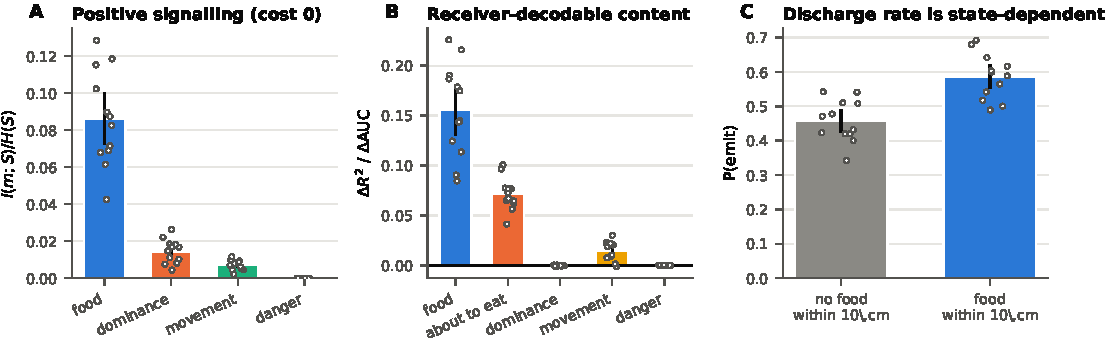
\includegraphics[width=\textwidth]{../figs/fig4_content.pdf}
\caption{\textbf{What the pulse train carries.} (A) Positive signalling,
conditioned on distance-to-neighbour decile. (B) Cross-validated decoding from
receiver-observable pulse counts only, minus the time-shifted baseline. (C)
Discharge probability by food proximity.}
\label{fig:content}
\end{figure}

\begin{figure}[t]
\centering
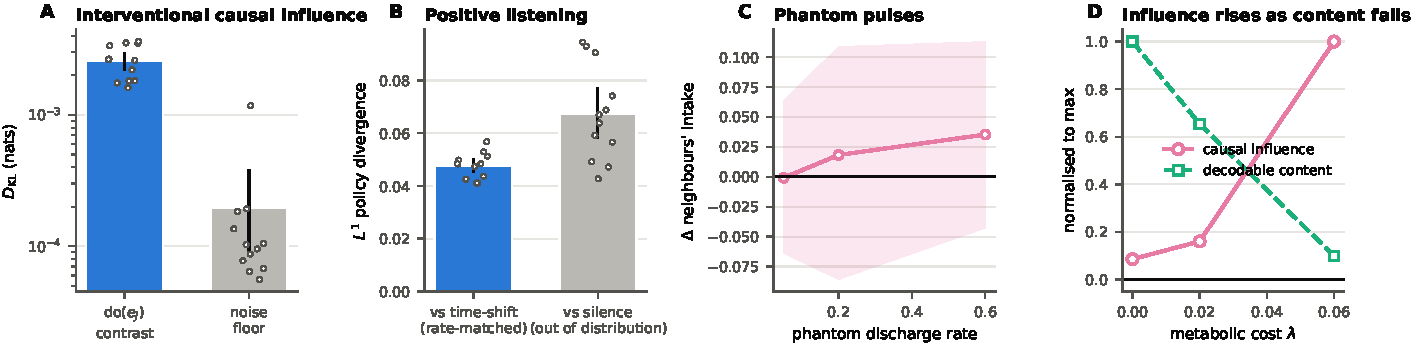
\includegraphics[width=\textwidth]{../figs/fig5_listening.pdf}
\caption{\textbf{Positive listening, and why it is not enough.} (A)
Interventional causal influence against its noise floor (log scale). (B)
Positive listening against a rate-matched time-shift null and against silence,
which is out of distribution. (C) Phantom-pulse dose-response on neighbours'
intake. (D) The dissociation: as metabolic cost rises, causal influence per
discharge \emph{increases} while the information a receiver can decode
\emph{falls}. Influence and informativeness move in opposite directions, so
neither substitutes for the other.}
\label{fig:listening}
\end{figure}

\subsection{\dots but it has no payoff consequence}

Positive signalling and positive listening are both satisfied, so on the
effect-based definition this is communication. The payoff test says otherwise.

Replacing an emitter's public train with the train the same policy produced in a
\emph{different arena}---identical marginal rate, burst structure and inter-pulse
statistics, no contingency with the receiver's actual world---changes neither
party's return. The same holds for temporal scrambling, for identity scrambling,
and for phantom pulses injected at rates from \num{0.05} to \num{0.6}
(Fig.~\ref{fig:listening}C). Because a non-significant difference is not evidence
of no difference, we report these as two one-sided tests against an equivalence
margin fixed in advance at \SI{5}{\percent} of the intact condition's own return:
\TOSTVERDICT

The contingency of the public channel, as opposed to its presence, is worth
approximately nothing to anybody. A receiver can read the emitter's situation off
its pulse train, and does adjust its policy when the train changes, but nothing
downstream of that adjustment shows up in what either fish eats.

\subsection{Cost and predation regulate the probe without creating a signal}

The reference model gives discharges no cost. Adding one produces a clean
dose-response: discharge probability falls monotonically from \EmitCostZero\ at
$\lambda=0$ to \EmitCostHigh\ at $\lambda=0.08$ (Fig.~\ref{fig:phase}).
Eavesdropping predation pushes it lower again at every cost, and mortality falls
with it, so crypsis works. Cooperative harvesting sustains a higher rate than
competition at matched cost.

We expected this to make the pulse train informative. A budget has to be spent
where it pays, and a schedule that allocates pulses to the moments that matter
should be more diagnostic of the emitter's state than a constant one. The
opposite happens. Information about food falls monotonically with cost, from
$\Delta R^2 = \ContentCostZero$ at $\lambda=0$ to \ContentCostHigh\ at
$\lambda=0.08$, and the same decline appears for every other target we decoded.
It survives normalising per pulse: informativeness per discharge falls from
\PSPerPulseZero\ to \PSPerPulseHigh. The learned response to a metabolic price is
a lower baseline rate, not a smarter schedule.

Silence behaves the same way. Discharge probability is essentially identical
whether or not a predator is within \SI{25}{\centi\metre} (difference
\SilenceDangerDiff), and danger is close to undecodable from the public channel
(\DangerAUC\ AUC above the time-shifted baseline). Agents manage their average
exposure rather than timing their gaps, which is what a prey animal that cannot
see the predator coming can do; our predator detects discharges at
\SI{60}{\centi\metre} but is itself passively detectable only at about
\SI{25}{\centi\metre}.

\subsection{Sender shaping, with reception held fixed}

Our first attempt at the production-side test compared populations trained with
and without knollenorgans, and gave $\mathrm{SSI}=\SSIDeafZero$ at zero cost.
That contrast is confounded, and in a way worth spelling out because it is easy
to make. Disabling knollenorgans removes \emph{reception}. It therefore asks
whether a fish behaves differently when it can hear others, not whether it
behaves differently when others can hear \emph{it}. The direction of the effect
gives the confound away: hearing populations discharge \emph{less} than deaf ones
(\EmitHearZero\ versus \EmitDeafZero), which is free-riding---a fish that can
hear its neighbours' probes cuts its own costly sampling---and not audience
design, which would push emission up or restructure it.

The yoked condition holds reception fixed and cuts audibility instead. Receivers
get knollen input with matched statistics, drawn from another arena, so no
sender's pulses reach anybody while every receiver still has a realistic social
input stream. Measured this way, sender shaping is \SSIYokeZero\ at zero cost
(Fig.~\ref{fig:ssi}A), and discharge rate is \EmitLiveZero\ live versus
\EmitYokeZero\ yoked. \YOKEDVERDICT

\begin{figure}[t]
\centering
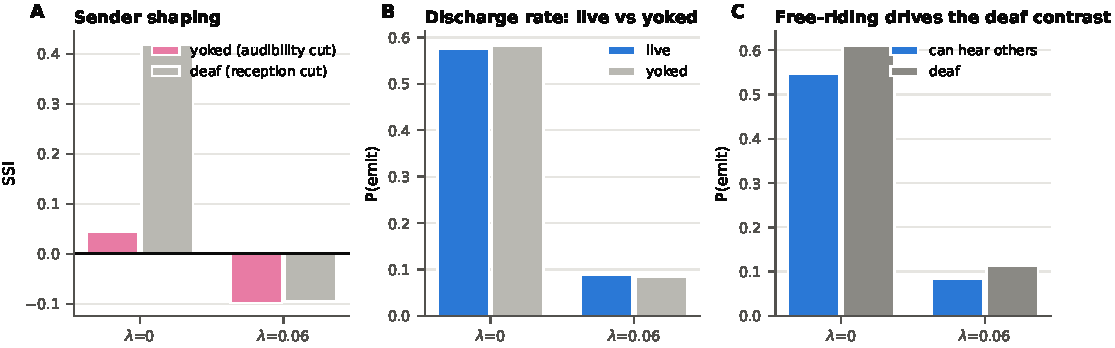
\includegraphics[width=\textwidth]{../figs/fig6_ssi.pdf}
\caption{\textbf{Sender shaping measured with reception held fixed.} (A) SSI from
the yoked contrast, which cuts audibility only, beside the confounded deaf
contrast, which cuts reception. (B) Discharge rate, live versus yoked. (C) The
free-riding effect that drives the deaf contrast: fish that can hear neighbours
discharge less.}
\label{fig:ssi}
\end{figure}

\subsection{A decoupled variable is what lets a social function appear}

A negative result is only as good as the positive control beside it, and to this
point every manipulation has left the discharge welded to its sensory function.
We therefore gave the agents a second variable: a discharge subtype, one bit,
that rides on the pulse---so sending still costs a pulse and still exposes the
fish to predators---but whose value changes nothing about the emitter's own
electric image, nothing about how the pulse illuminates neighbours, and nothing
about detectability. Only the content is decoupled, not the act.

\DECOUPLEDRESULT


\subsection{The same decomposition in a world with no electric fish in it}

If the result is about dual-use action channels rather than about
electroreception, it should reappear wherever an action senses and broadcasts at
once. We built a minimal environment with no fish physics in it: agents forage in
a unit square, and a \textsc{ping} action has exactly the three consequences a
discharge has---it shows the pinger the items near itself, it shows nearby others
the items near \emph{them}, and it is registered by everyone as an event with a
bearing. A weak always-on passive sense means silencing an agent is not the same
as blinding it. The same masks, the same trainer and the same intervention battery
apply unchanged.

The decomposition replicates. Agents that can ping collect \DUFull\ items per
episode against \DUSilent\ for permanently silent ones; muting one agent costs it
\DUTotal\ items, of which \DUPriv\ (\DUPrivFrac\%) is its own lost reafference and
\DUSig\ its lost detectability (Appendix~\ref{app:dualuse}). Pricing the ping
suppresses it from \DUPingLo\ to \DUPingHi. Neither the sign nor the rough
magnitude of the decomposition depends on the electric-fish biophysics; what it
depends on is that one action does two jobs.


\subsection{The regime map, and how far it generalises}

Appendix~\ref{app:regimes} gives the full cost $\times$ predation $\times$
economics grid and the rule-based regime labels. The structure
is orderly, but it is the structure of a probe schedule being turned up and
down: the axes that move are discharge rate and mortality, while the
informational and payoff-relevance axes stay near zero throughout.

\GENERALISATION

\begin{table}[t]
\centering\small
\caption{The muting decomposition across scales and architectures. ``Private share'' is the fraction of the total muting effect attributable to the emitter's own lost reafference.}
\label{tab:gen}
\begin{tabular}{lrrrrr}
\toprule
Condition & seeds & total & $-$reafference & $-$detection & private share \\
\midrule
baseline (4 fish, 60\,cm, 512 steps) & 12 & -0.40 & -0.40 & +0.11 & 101\% \\
2 fish & 6 & -1.66 & -1.58 & -0.02 & 95\% \\
6 fish & 6 & -0.43 & -0.59 & -0.08 & 135\% \\
100\,cm arena & 6 & -0.31 & -0.34 & -0.02 & 107\% \\
1024-step episodes & 6 & -1.10 & -0.92 & +0.08 & 83\% \\
256-unit GRU & 6 & -0.61 & -0.57 & +0.11 & 93\% \\
\bottomrule
\end{tabular}
\end{table}


